\documentclass[addpoints, 11pt]{exam}

\usepackage{amsmath}
\usepackage{amssymb}
\usepackage{graphicx}
\usepackage{hyperref}
\usepackage{fancyhdr}

\pagestyle{fancy}

\rhead{{\bf Assigned:} April 1, 2015 \\{\bf Due:} Week of April 20, 2015}

\printanswers
%\noprintanswers
\newcommand{\ds}{\displaystyle}
\newcommand{\lm}{\lim\limits}
\newtheorem{Definition}{Definition}

\begin{document}
\vspace{100mm}
\begin{center} \Large
MTH 371: Group Project 3 \\ Cubic Splines \normalsize
\end{center}
\ \\
\noindent GENERAL GROUP PROJECT GUIDELINES: 
\begin{itemize}
\item Group project assignments should be a collaborative effort. All should participate in discussion and solution writing. \vspace{-2mm}
\item Two weeks after the project is assigned, your group will meet with Dr. Vidden to discuss. All members must be present. Your grade will be determined at the end of the meeting. \vspace{-2mm}
\item Each student should keep group project solutions in a dedicated notebook. Bring this notebook to your weekly meeting to discuss your findings. For coded solutions, bring a laptop to your weekly meeting. Have the laptop ready before the start of the meeting. \vspace{-2mm}
%\item Clearly label all plots (title, $x$-axis, $y$-axis, legend). Use the \verb1subplot 1command when comparing 2 or more plots.
\end{itemize}
\ \\

Cubic splines are used extensively in a wide range of applications from Boeing designing airplanes to Pixar creating animated films. Check the papers on D2L for some details on this process. With this project, you will see the implementation of cubic splines as a way to model everyday shapes.

\begin{questions}

%%%%%%%%%%%%%%%%%%%%%%%%%%%%%%%%%%%%%%%%%%%%%%%%%%%%%%%%%%%%%%%%%%%%%
\question Make a plot of one of your group member's hand with Scilab. To do this, start with \\ \ \\
\texttt{z=locate();} \\
\texttt{x=z(1,:)';} \\
\texttt{y=z(2,:)';} \\ \ \\
The return is a sequence of points as you clicked them. Read the documentation for \verb1locate()1 for details. Use \verb1plot(x,y)1 to check your data.

%%%%%%%%%%%%%%%%%%%%%%%%%%%%%%%%%%%%%%%%%%%%%%%%%%%%%%%%%%%%%%%%%%%%%
\question Note, the curve which we will fit to these points is not a function. Hence, we create a parametric spline. Translate the attached Matlab function \verb1splinetx(x,y,u)1 to Scilab. Running the following script, create a spline-fitted outline of your hand. Make sure you completely understand this function you are rewriting and how parametric splines work. On the reverse page, I have include a resulting picture for my own hand!\\ \ \\
\texttt{n = length(x);} \\
\texttt{s = (1:n)';} \\
\texttt{t = (1:.05:n)';} \\
\texttt{u = splinetx(s,x,t);} \\
\texttt{v = splinetx(s,y,t);} \\
\texttt{xdel(winsid());} \\
\texttt{plot(x,y,'.',u,v,'-');}

%%%%%%%%%%%%%%%%%%%%%%%%%%%%%%%%%%%%%%%%%%%%%%%%%%%%%%%%%%%%%%%%%%%%%
\question Use your handy data coupled with the built in Scilab function \texttt{splin}. Fit three types of splines to your data, not-a-knot, clamped, and natural. What differences do you see? Research these types of splines more to confirm the differences you see. 
\pagebreak

%%%%%%%%%%%%%%%%%%%%%%%%%%%%%%%%%%%%%%%%%%%%%%%%%%%%%%%%%%%%%%%%%%%%%
\question BONUS extra credit problems. 
\begin{parts}
\part Rewrite the \texttt{splinetx} function to suit the clamped and natural spline conditions.
\part Devise your own artistic spline creation using the above methods.
\part Download the secret project 3 Scilab files from D2L and apply the above ideas to improve the result.
\end{parts}

\begin{center}
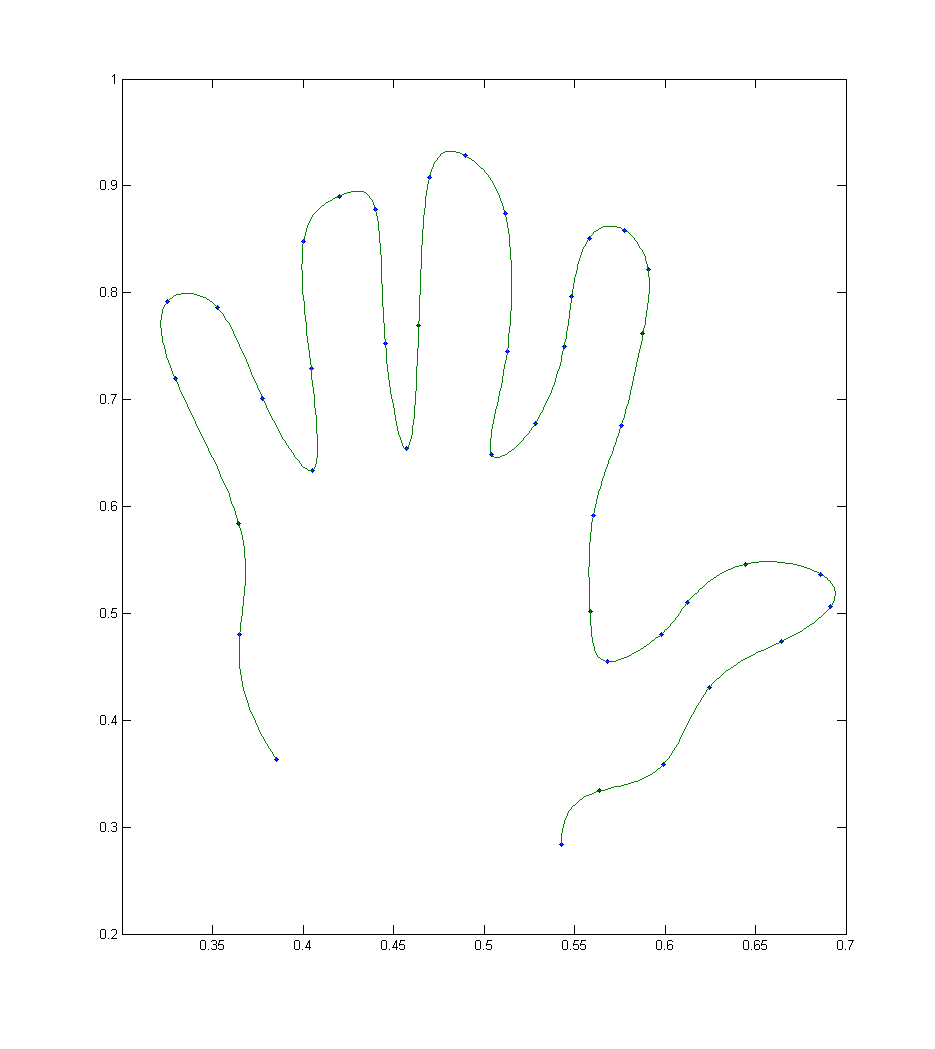
\includegraphics[width=3.5in]{myhand.png} 
\end{center}

\end{questions}
\end{document} 